\chapter{Optical Lens Design}
\label{chapter_LensDesign}
\graphicspath{ {./chapter-sp/figures/} }
\captionsetup[figure]{labelfont=bf}
\captionsetup{margin=1.5em}
\captionsetup[table]{labelfont=bf}

\epigraph[0pt]{
Successful design will require the application of individual creativity as well as artful manipulation and thorough comprehension of the numeric tools available in lens design programs.\cite{book:Shannon1997}
}{R. R. Shannon}


In this chapter, we start with a simple example of how a magnifying glass can be designed on paper (instead of on a computer). This section is added since nowadays the design is mostly done with professional software and the story of how a lens can be designed from scratch based on theory, is less clear. After that, we explain the modern optical approach with an emphasis on optimization techniques. The SPC method is briefly mentioned at the end of the chapter in comparison with other design/optimization techniques and it is elaborated in the next chapter. 

%%Definition of optical design
\section{Designing a Magnifying Glass}

%Useful reference, https://opentextbc.ca/universityphysicsv3openstax/chapter/the-simple-magnifier/%
\vspace{1em}
We use a simple magnifying glass as an example to demonstrate the basic approach of lens design. As the name suggests, a magnifying glass magnifies objects and is commonly used to assisting reading when the letters are too small to read. Assume the magnification requirement of the magnifier is $6\times$. We know from text book \cite{hecht2012optics} that such a magnifier can be made using a convex lens. The magnified image is a virtual image that is then captured by the human-eye. The magnification of a magnifier is defined as the angular magnification which is the ratio between the subtended angles to the eye of the object and the image. This is illustrated in Figure \ref{fig: geo_formulae}-a. A larger angle means a larger image is formed on the retina of the eye. The object and image are normally located at a distance of $250 mm$ from the eye. The distance represents the near-point, which is the closest distance that the eye can view comfortably. 
% illustration of the angular magnification[done]


Figure \ref{fig: geo_formulae}-b shows how the virtual image is formed considering an ideal thin lens scenario. Certain rules are used to derive such a plot:
1) A light ray, which starts from the object plane and is parallel to the optical axis, will pass the focal point at image side;
2) A light ray, which starts from the object plane and passes the nodal point (the intersection between the ideal lens and the optical axis), will remain its original direction.

In this thesis, we use the following convention for the geometrical optics formulas: points (object, image or focal point) sitting on the left side of the lens has a negative distance to the lens. Points sitting on the right side of the lens has a positive distance. The radius of the optical surfaces is positive when the center of curvature is to the right of the surface vertex, and vice versa. 

\begin{figure}
    \centering
    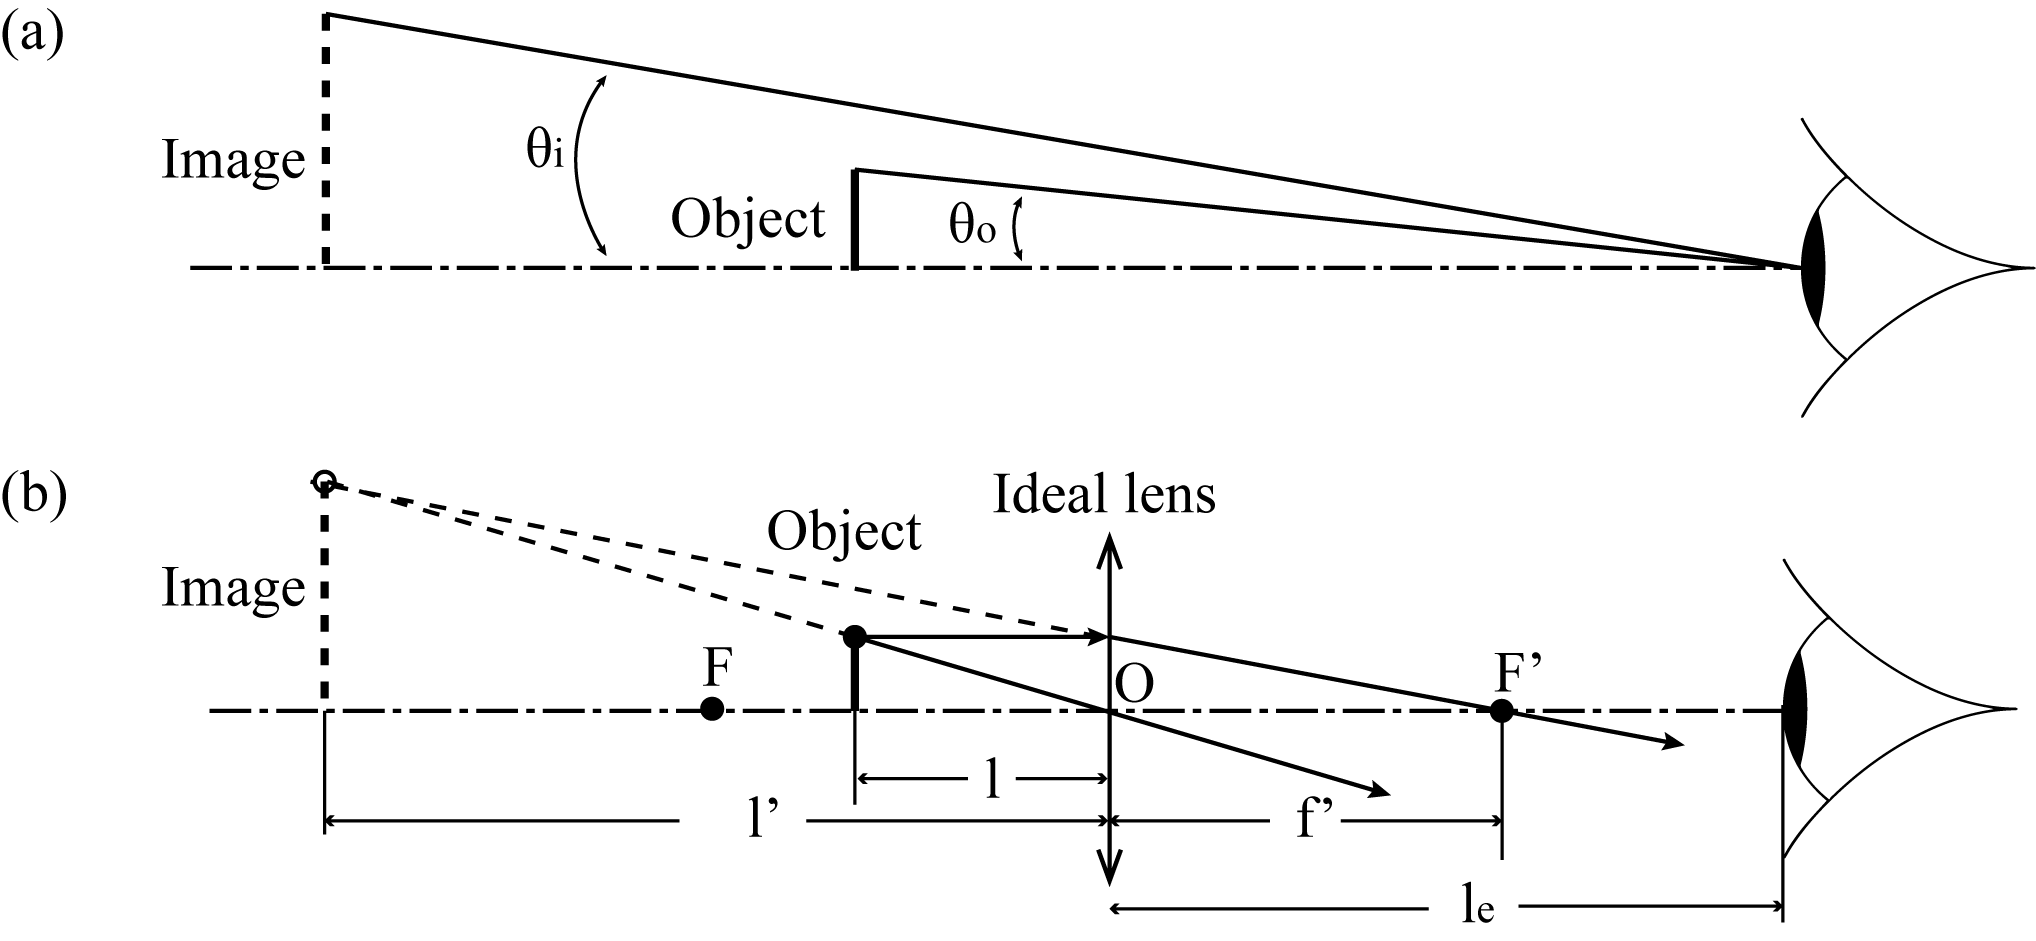
\includegraphics[scale=0.58]{chapter-1/figures/geo_magnifier_v2.png}
    \caption{(a) The magnification of a magnifying glass is defined as the ratio between the image subtended angle $\theta_{i}$ and  the object subtended angle $\theta_{o}$.  
    (b) Illustration of a virtual, enlarged image of the object through a magnifying glass. Equations \ref{eq: thinlensformula} - \ref{eq: magnifier magnification} explain the relation of the parameters.}
 %(b) Illustration of the Lensmaker's equation. For thin lens case, the equation is given by \ref{eq: lensmaker_r}. The thick lens case equation is given by \ref{eq: lensmaker_r_thick}.[old caption]
    \label{fig: geo_formulae}
\end{figure} 

The subtended angle $\theta_o$ of the object to the eye writes 
\begin{equation}
\label{eq: magnifier object angle}
\theta_o = \frac{h_o}{250 \; \text{mm}},
\end{equation}where $h_o$ stands for the height of the object.
The subtended angle $\theta_i$ of  the magnified image writes
\begin{equation}
\label{eq: magnifier image angle}
\theta_i = \frac{mh_i}{l_e-l'},
\end{equation}where $m (= \frac{l'}{l})$ is the lateral magnification and $l_e$ is  the distance from the eye to the lens. Since the image is virtual ($l'<0$), the expression $l_e - l'$ indicates the distance between the image and the eye. Together with the thin lens equation 
\begin{equation} \label{eq: thinlensformula}
    \frac{1}{l^\prime} - \frac{1}{l} = \frac{1}{f^\prime},
\end{equation}we can write Equation \ref{eq: magnifier image angle} into
\begin{equation}
\label{eq: magnifier image angle reform}
\theta_i = (1-\frac{l'}{f'})\cdot\frac{h_o}{l_e-l'}.
\end{equation}With Equation \ref{eq: magnifier object angle} and Equation \ref{eq: magnifier image angle reform}, the magnification $m_{mag}$ of the magnifier is 
\begin{equation}
\label{eq: magnifier magnification}
m_{mag} = \frac{\theta_i}{\theta_o} = (1-\frac{l'}{f'})\cdot\frac{250 \; \text{mm}}{l_e-l'}.
\end{equation}The distance between the image and the eye $l_e-l'$ can be set as $250 $ mm. For the maximum $m_{mag}$, we have $l' = -250 \; \text{mm}, l_e \approx 0$. It means that when the eye is observing close to the magnifier, the maximum magnification of the image is achieved. This magnification is
\begin{equation}
\label{eq: magnifier magnification simplified}
m_{mag}  = 1+\frac{250 \; \text{mm}}{f'}.
\end{equation}Now we substitute $m_{mag}$ with $6$, then we have $f' = 50 $ mm. As a result, we need a magnifying glass with a focal length of $50 $ mm to achieve a magnification of  $6\times$.
%% use the following equation to derive lens shape 2021-09-28 [done]
Now we know the focal length  $f' = 50 $ mm and the image distance $l' = -250 $ mm. Given Equation \ref{eq: thinlensformula}, the object distance is calculated to be $41.67 $ mm.  

For a spherical lens, the radii of the two spherical surfaces of the lens can be calculated using Lensmaker's equation 
\begin{equation} \label{eq: lensmaker_r}
    (n-1)(\frac{1}{R_1} - \frac{1}{R_2}) = \frac{1}{f^\prime},
\end{equation}
where $n$ stands for the refractive index of the lens material. $R_1$ and $R_2$ are the radii of the two spherical surfaces. The focal length $f^\prime$ is $50 $ mm. Let us use a common optical material such as BK7 glass. It has a refractive index ($n$) of approximately $1.5$ in the visible spectrum. For simplicity, we use $1.5$ as our refractive index value.

Now in Equation \ref{eq: lensmaker_r}, the two radii can still vary and we do not have a unique set of values to satisfy the equation. We can choose to have a double-convex lens by forcing the absolute radii to be identical, where $R_1 = 50 $ mm, and $R_2 = -50 $ mm. 

Equation \ref{eq: lensmaker_r} assumes the thickness of the lens is very small compared to the radius of the two surfaces (a thin lens scenario). There is also the equation when the thickness $d$ of the lens is considered:
\begin{equation} \label{eq: lensmaker_r_thick}
    (n-1)\left( \frac{1}{R_1} - \frac{1}{R_2} + \frac{(n-1)d}{nR_1R_2} \right) = \frac{1}{f^\prime}  .
\end{equation}
With a thickness $d$ of $3 $ mm, the radii can be now calculated using Equation \ref{eq: lensmaker_r_thick} to be$R_1 =  49.50 $ mm and $R_2 = -49.50 $ mm. These values are very close to the case when using thin lens approximation ($50 $ mm and $-50 $ mm). 
At this phase, the above derivation shows that based on first order (Gaussian) optics, the following specification can achieve a magnification factor of $6\times$, given that the object locates $41.67 $ mm from the lens:

\begin{table}[h!]
    \centering
    \captionsetup{justification=centering}
    \caption{Magnifying Lens Specification}
    \label{magnifying lens specs}
    \vspace{-1em}
    \begin{tabular}{ p{15em}  c }
    \hline 
    Magnification & $6\times$\\ 
    Number of lens & $1$\\ 
    Diameter (mm) & $20$ \\ 
    Refractive index & $1.5$\\ 
    Thickness (mm)& $3$\\ 
    Radii (mm) & $49.50$, $-49.50$\\
    Effective Focal Length (EFL, mm) & $50$\\
    \hline
    \end{tabular}
\end{table}
 
For the aforementioned example, we used the most basic Lensmaker's formula to design a $6 \times$ magnifier with a double-convex lens.  The condition of double-convex is chosen by us since according to Equation \ref{eq: lensmaker_r_thick}, there are infinite choices of radii that satisfy the equation. Note that the Lensmaker's formula is based on first-order optics, where the angle between the rays and the optical axis is assumed to be very small. This assumption does not hold anymore when optical aberration needs to be treated. In the following part, we show an example on how to improve the magnifier design considering minimizing the spherical aberration. An illustration of spherical aberration is given in Figure \ref{fig: spherical aberration}. Light rays emit from an on-axis point and their deviation from the expected refracted\footnote{For a mirror, it is reflected.} on-axis point is called spherical aberration. 
\begin{figure}
    \centering
    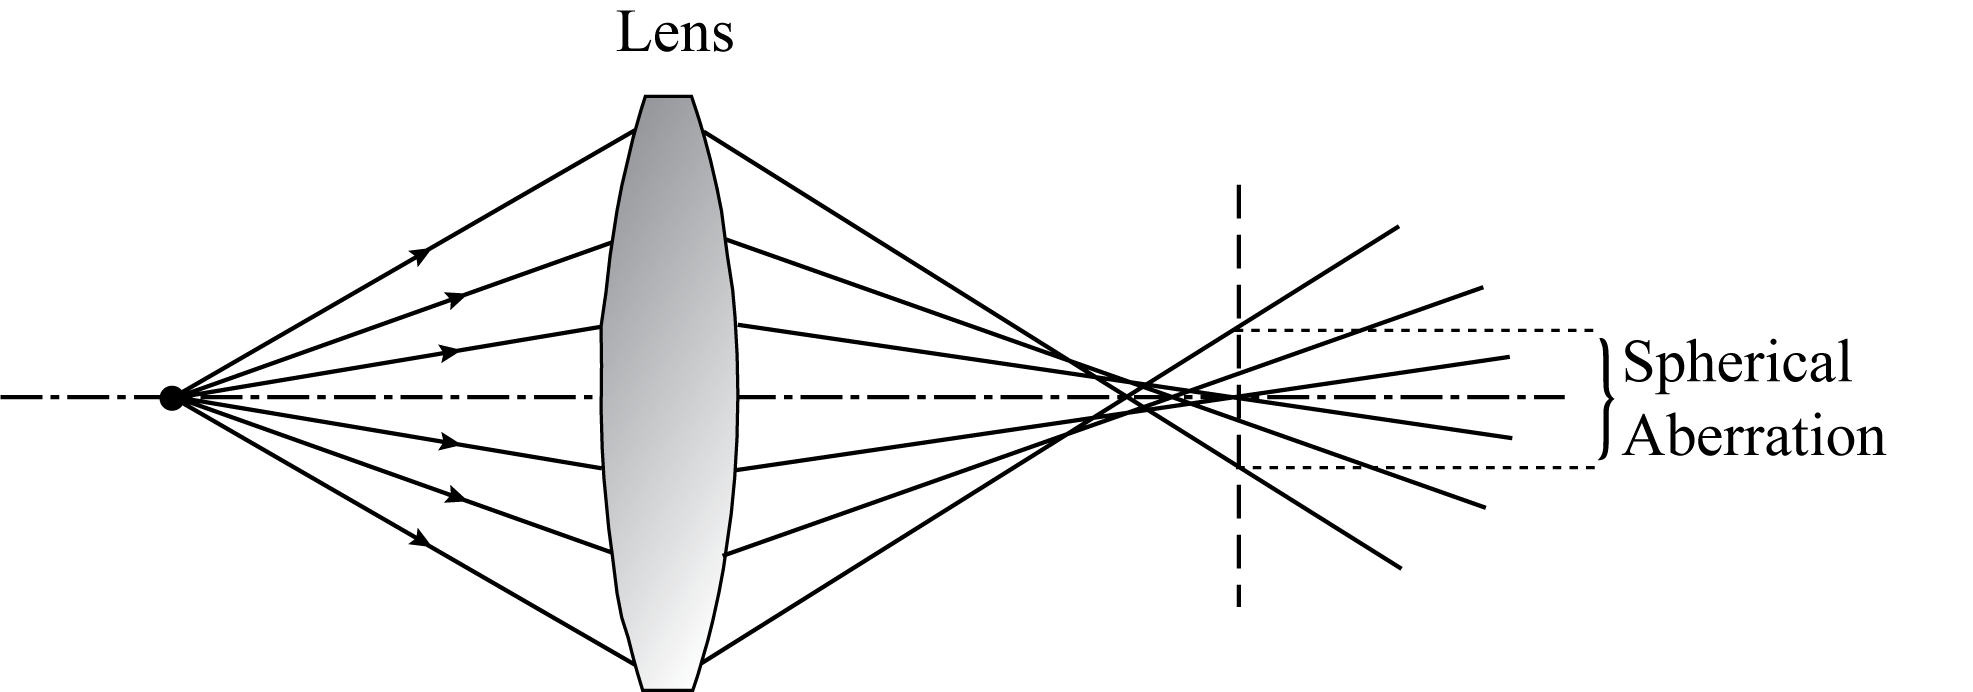
\includegraphics[scale=0.58]{chapter-1/figures/illus_spherical_abe.png}
    \caption{Illustration of the spherical aberration in the optical system. The light rays emitting from one on-axis object point is not converging perfectly into one on-axis point on the image plane. The deviation from the expected on-axis point is called spherical aberration.}
    \label{fig: spherical aberration}
\end{figure} 
The primary monochromatic aberration are the spherical aberration, coma, astigmatism, field curvature and distortion. There are axial and lateral chromatic aberrations when chromatic application is considered. Given the thin lens model, the coefficient of each aberration term can be explicitly expressed. The term of the spherical aberration can be expressed as (\cite{GrossHBOvol1}, 29.4.7):
\begin{equation} \label{eq: Si_spherical}
    S_I = \frac{h^4}{4{f^\prime}^3}\left(\frac{3n+2}{n}M^2 - \frac{4(n+1)}{(n-1)n}XM + \frac{n+2}{(n-1)^2n}X^2 + \frac{n^2}{(n-1)^2}\right).
\end{equation}                            %% Figure illustration of the spherical aberration. I don't think I need to add it. 21/09/18%[done]
where $h$ indicates the ray height on the lens surface. $X$ stands for the bending factor of the thin lens (\cite{GrossHBOvol1}, 10.1.1):
\begin{equation} \label{eqn: bending factor}
X = \frac{R_1+R_2}{R_2-R_1},
\end{equation}and $M$ stands for the position parameter (\cite{GrossHBOvol1}, 10.1.2):
\begin{equation} \label{eqn: position parameter}
M = \frac{1+m}{1-m},
\end{equation}$m$ is the magnification factor and it is $6$ as defined previously. In this case, $M=-\frac{7}{5}$. In Equation \ref{eq: Si_spherical}, for a chosen ray, parameter $f^\prime$, $M$, and $n$ are all given. Therefore, $S_I$ becomes a quadratic function for the bending factor $X$. There is a value of $X$ that minimize the value of $S_I$. In this case, when $X = -1$ , the minimum value of $S_I $ is $ 8.16(\frac{h^4}{4(f^\prime)^3})$. The spherical aberration of each ray is proportional to its ray height given the fixed lens configuration. 

Now if we consider both the Lensmaker's Equation \ref{eq: lensmaker_r} and the spherical term in Equation \ref{eq: Si_spherical}, the two radii of the lens can be solved as $R_1 = \infty, R_2 = -25$ mm. These two values are very different from the values ($50$ mm and $-50$ mm) calculated based on first-order optics. It is worth mentioning that Equation \ref{eq: Si_spherical} assumes a thin lens, hence the comparison of the radii is done between thin lens models. It is also observed that in our magnifier example, considering a $3$ mm lens thickness in Lensmaker's formula does not alter the radii significantly.  

When more aberration terms are considered, the number of variables in this example is not enough to analytically solve the values for the minimal values of each aberration term. Normally, new degrees of freedom will be introduced to the system (e.g. adding new lenses). However, more number of variables also implies an increasing complexity of the formulae. Modern optical design handles it by using computer-aided design techniques. Numerical optimization and rapid ray tracing are done by computers, which improves the efficiency of optical design.  


\section{Modern Optical Design}
\vspace{1em}
Prior to the development of digital computers, lens optimization was a hand-calculation task using trigonometric and logarithmic tables to plot Two-Dimensional (2D) cuts through the multi-dimensional space. As the development of the digital computer in the 20th century, it drastically shapes the way how optical design is being practised. The burden of calculation is tremendously reduced by using computers. Instead of calculating each ray path on paper,  optical systems are parameterized into different variables representing the physical construction of an optical system (a physical model). For example, a simple two-element air-spaced spherical lens can be represented with nine variables (four radii of curvature, two thickness one airspace, and two glass types). With increasing complexity (number of elements, type of surfaces) of the system, the number of variable can reach hundreds. Using modern computers allows rapid ray tracing calculation by which the performance of the lens system can be quickly modelled and evaluated. 

Helped by the technique of numerical optimization, the vast high-dimensional design space can be searched to look for the set of variables providing the optimal performance of the system. Lens optimization has been studied as early as the 1940s \cite{wikilensdesign}. The earliest attempt for optimizing a doublet using computer dates back to 1950s, when James G. Baker used the \textit{Harvard Card Programmed Calculators} \cite{ThompsonOpticalDesignHistory}.  A good description of the starting of computer-aided optical design is given in a 1963 paper by Feder \cite{Feder:63}. In order to optimize an optical system using the computer, a merit function is necessary to be constructed. The value of this merit function predicts the performance of the system. Normally, the smaller the value of the merit function, the better the performance should be. For an imaging system, such a merit function can be the sum of the aberrations, the size of the focused spot, etc.  The merit function in optical design is commonly defined as \cite{GrossHBOvol3}:
\setlength{\belowdisplayshortskip}{5pt}
\setlength{\abovedisplayshortskip}{5pt}
\begin{equation} \label{eq:MFdefi}
MF(\pmb{x})=\sum_{j=1}^{m} w_j [\tilde{f}_j(\pmb{x}) - \tilde{f}_{tar,j} ]^2,
\end{equation}
\noindent where $\textbf{x} = (x_1, x_2, ..., x_N)$ is a vector describing a point in the $N$-dimensional variable space. $\tilde{f}_j(\textbf{x})$ are the operands with target values $\tilde{f}_{tar,j}$. $\tilde{f}_j(\textbf{x}) - \tilde{f}_{tar,j}$ could be defined as elementary aberration such as ray or wavefront deviations for selected rays. $w_j$ are the positive weighting factors, therefore $MF$ is a single number giving the residual of various operands and their target values. The weights and targets can be absorbed in the definition of the operands, therefore we have 
\begin{equation} \label{mf_oprand_vector}
MF(\pmb{x}) = \pmb{f}^{T}(\pmb{x})\cdot \pmb{f}(\pmb{x}),
\end{equation} where $\pmb{f}$ is a vector having the operands as components.

Given the merit function, a high dimensional space is determined. Each sets of value of the variables represents a point in this high dimensional space and the value of the merit function is determined at that point. Ideally, the value of the merit function is directly associated with the performance of the optical system is being designed. The minimal value of the merit function is desired because it represents the best system performance. 

Once the variables are chosen from the system, the next step is to apply numerical optimization techniques to minimize the value of the merit function defined in Equation \ref{eq:MFdefi}:
\begin{equation} \label{eq:MFopt_cp1}
\begin{split}
& \text{minimize}\;\; MF(\pmb{x}) ,\\
& \text{subject to some constraints},
\end{split}
\end{equation}
with optimization, a new set of values of the variables $\pmb{x_{opt}}$ is obtained such that the value of the merit function is a minimal.

As shown in the example of the magnifier, in order to fulfill the requirements of working distance, magnification and at the same time minimize the spherical aberration for a thin lens model, the radii of the optical surfaces have been calculated. However, in practice, spherical aberration is not the only aberration contributor that limit the image performance. At the same time, some thickness of the lens needs to be added for practical reasons. Given the previously calculated radii and other parameters of the magnifier, a merit function value can be determined after the lens is modeled in an optical design software. This merit function value usually can be further reduced for better system performance with optimization techniques.  

We applied optimization for the previous magnifier example in optical design software CODE V. Three different cases are parameterized in CODE V as starting points for the optimization. They are calculated using the Lensmaker's formula  (Equation \ref{eq: lensmaker_r}), Lensmaker's formula considering a thick lens (Equation \ref{eq: lensmaker_r_thick}), and the spherical aberration formula for a thin lens (Equation \ref{eq: Si_spherical}). The variables are the two radii of the surfaces. The thickness is also used as a constrained variable to optimize for a thick lens configuration. The radii and merit function in each step of the optimization of the three cases are listed in Table \ref{tb: magnifier optimization}. 
% to do: 1) to add the merit function in the table[done].  2) good to have, to have the plot of the systems [not necessary to do]
% the magnification of the magnifier is the defined typically as the angular magnification, so the model need recalcualtion, but the process should be the same !!!!!!! 09/23. Need further continuation on the topic after fix the magnification definition [done] 

In CODE V, the object distance is set as $41.67 $ mm and the image distance is at $250 $ mm. An EFL of $50 $ mm is used as a constraint of the system. Only one wavelength is used and the material refractive index is set as $1.5$. An entrance pupil diameter of $20 $ mm is used and the fields are defined with three object heights: $0$, $3$, and $5 $ mm.  The merit function used here is the default transverse-ray function in CODE V. It is a composite value, scaled so that it is the mean square of the weighted image radius.

When optimized directly with the input setting, the starting points of both thin lens approximation using paraxial optics and the one optimized for spherical aberration converge to the same local minimum (radii are given in the "Optimized thin" column in Table \ref{tb: magnifier optimization}). We also notice that the starting point for the thin lens which is optimized for spherical aberration already has very similar radii comparing to the CODE V optimized system. It indicates that for such a configuration, the image quality is dominated by the spherical aberration and the theoretical calculation predicts the image quality well. However, it is also noticed that the merit function value of these systems are very big ($9.06E5$ \textmu m$^{2}$). Here we use this example only to demonstrate how a simple lens design and optimization flow works. In practical design, the merit function value needs to be further brought it down and additional degrees of freedoms (such as new lenses) are required. 

We also optimized the system with a lens thickness constrained at $3 $ mm. Three starting points all converge to the same local minimum. It indicates that there is no difference which starting configuration we choose. We will show later in the thesis that it is not the cases for more complicated optical system (e.g. with more lenses). 
% what I want to show 1) how a flow of modern design is 2) it is a simple case.
\newcolumntype{M}[1]{>{\centering\arraybackslash}m{#1}}
\begin{table}[h!]
	\small
    %\centering
    \captionsetup{justification=centering}
    \caption{Optimization results of the magnifying glass in CODE V}
    \label{tb: magnifier optimization}
    \vspace{-1em}
    \begin{tabular}{|M{2cm}|M{0.9cm}|M{0.6cm}|M{0.8cm}|M{0.8cm}|M{0.6cm}|M{0.8cm}|M{0.8cm}|M{0.6cm}|M{0.8cm}|}
    \hline
  &\multicolumn{3}{c|}{\textbf{Starting point}} & \multicolumn{3}{c|}{\textbf{Optimized thin}} & \multicolumn{3}{c|}{\textbf{Optimized thick}}\\ \cline{2-10}
  &  Radii (mm) & THK (mm) & MF (\textmu m$^{2}$)&  Radii (mm) & THK (mm) & MF (\textmu m$^{2}$) &  Radii (mm) & THK (mm) & MF (\textmu m$^{2}$)     \\  \hline
   \textbf{Thin lens }  & 50, -50 & 0 & 3.56E6 & 2247, -25 & 0& 9.06E5&&&\\ \cline{1-7}
    \textbf{Thick lens} & 49.50, -49.50& 3 & 6.45E6 & /&/&/&  \multirow{3}{*}{108, \newline -32} & \multirow{3}{*}{3} &\multirow{3}{*}{4.98E6}\\ \cline{1-7}
    \textbf{Thin lens optimized for SA} & $\infty, -25$ & 0 & 9.07E5 & 2247, -25&0&9.06E5&&&\\ 
    \hline
    \end{tabular}
    \footnotesize{THK: thickness. SA: spherical aberration.}
\end{table}

In summary, the process of the modern optical lens design can be simplified into two steps: 1) determine parameterized configurations of the system as starting points; 2) use optimization tools to optimize the system performance. In practice, the two steps can be iterated for many times to finally obtain a satisfactory system. Mastering both steps requires a good understanding of the optical systems as well as in-depth knowledge of optimization. We will explain these two parts in the following sections, with an emphasis on the optimization techniques. 

\subsection{Optical System Optimization }
\vspace{1em}
When the optical system and its merit function are treated as an optimization problem, there are two kinds of situations: 1) the merit function is a \textit{convex} function \footnote{Geometrically, a function is \textit{convex} if a line segment drawn from any point $(\pmb{x}, f(\pmb{x}))$ to another point $(\pmb{y}, f(\pmb{y}))$ -- called the \textit{chord} from $\pmb{x}$ to $\pmb{y}$ -- lies \textit{on or above} the graph of $f$.} and there is only one global minimum; 2) the merit function is a \textit{non-convex} function and there are multiple local minima. 

Simple cases such as the Magnifier example, the spherical aberration is a quadratic function of the bending factor.  The given number of equations equals the number of variables. An extract solution can be solved. However, in optical design, the common situation is that the number of equations is larger than the number of variables \footnote{In terms of ray tracing, each ray becomes an equations of the given variables. Hundreds of rays are normally traced for calculating the merit function.}. In this case, an approximation of the solution can be given. This is achieved by local optimization, where one minimum can be acquired. 

It is also observed that when the number of the variables (e.g. the number of lenses) increases, the number of the solutions also increases \footnote{A good example is illustrated in Page 61 of Reference \cite{vanTurnhoutThesis2009}. The contour plot of the merit function of a doublet with respect to two variables shows four local minima.} This is because the merit function becomes \textit{non-convex} as the variable increases. The results of the local optimization is then sensitive to the initial point where optimization starts.  

\subsubsection{Basins of Attraction \label{label: basinOfattrac}}
\vspace{1em}
In an optimization problem, the basin of attraction defines a set of points in the optimization space, where the optimization leads to the same local minimum. An example of a one-dimensional merit function and its corresponding basins of attraction is given in Figure. \ref{fig: basinOfattraction}. 

\begin{figure}
    \centering
    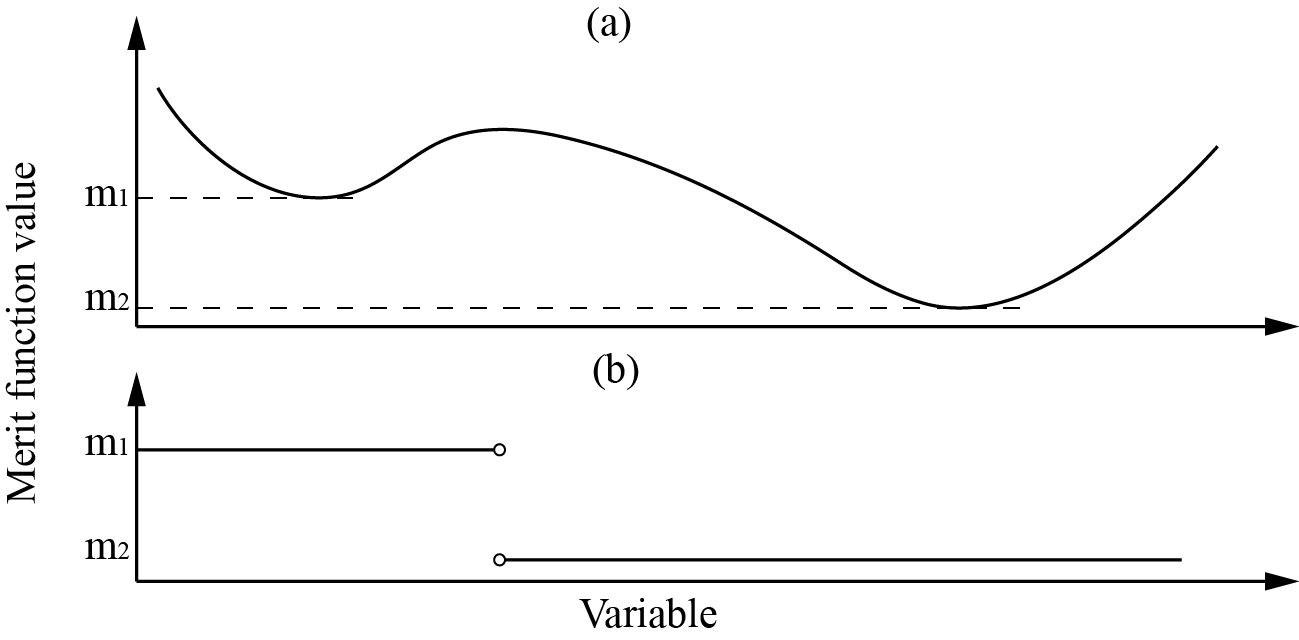
\includegraphics[scale=0.58]{chapter-1/figures/basinOfattraction.png}
    \caption{Illustration of basins of attraction in a one-dimensional optimization space. (a) The merit function with two local minimum having value $m_1$ and $m_2$ . (b) The corresponding basins of attraction in the plotted merit function region. At the boundary of the two basins, it is unclear where the optimization leads to, therefore marked as circles.}
    \label{fig: basinOfattraction}
\end{figure} 

The illustration of the basin of attraction is a direct way to visualize how optimization results in the optimization space, especially in a non-convex problem \footnote{In Chapter 4, basins of attraction on the two-dimensional hyper-plane are used for demonstration purpose. }. The result of a local optimizer is determined by its starting point. Since the goal of this problem is to find the global minimum among the many, there are two consequent strategies: 
1) start from the basin of attraction that corresponds to the global minimum; 
2) search for all (most of) the basins of attraction, list all the minima and obtain the global minimum.

In optical design, the former one is largely associated with the conventional optical design strategies. The starting point can be determined from the literature and patent data, where the system is believed to have a larger chance to lead to a satisfactory minimum. Another approach is to compute the system parameters based on analytical model. The assumption is that the starting point provided by the analytical model is in the basin of attraction of the global minimum.  However, when the optical system becomes increasingly complicated, e.g. adding lenses, making surfaces aspheric, etc., it is very difficult to fully analysing the system and providing a starting point. The strategy of finding multiple minima and selecting the best among them becomes more preferred in this situation. 

The most straightforward method to search for the global minimum is to systematically evaluate the merit function value on the multi-dimensional grid. The problem of this method is that the computational time increases exponentially with the number of variables. By applying a local optimizer, the amount of merit function evaluations can be reduced when starting from a basin of attraction. The task of finding the global minimum is then transformed to finding the basin of attraction containing the global minimum. 

\subsection{Getting the Starting Point}
When multiple minima presented in the optical design space, the result of the local optimization is sensitive to its choice of the starting point. In the conventional optical design practice, large effort is spent on obtaining a good starting point. 

As demonstrated in the beginning of this chapter, simple systems such as the Magnifier can be computed using first-order optics and third-order aberration model to obtain a relative good starting point. For more complicated systems which contain more optical elements and difficult requirement, there are design strategies summarized by lens designers based on their in-depth knowledge and extensive experience \cite{LivshitsQA2013}\cite{Shafer1995_moreless}. However, mastering these design methods can require years of practice.   

A common practice is that optical designers scan through the existing catalog of the available designs. This can be via patent search or by looking up examples in the optical design books \cite{smith1992modern} \cite{book:SmithModernOpticalEngineering}.  The one has the closest specification with respect to the design requirement is chosen to serve as the  starting point of the design. The assumption is that this chosen system is already in the basin of attraction where good system performance is expected. By doing some fine adjustment, the preferred system should be achievable. 

Methods such as Simultaneous Multiple Surface (SMS) method \cite{MinanoOE09}, which obtains a starting point based on iterative ray tracing process, have also been getting many attentions recently. The SMS method can be very effective for obtaining starting points consisting of aspherical lenses. In Chapter \ref{chapter_5_SMS}, we will look at the SMS method and the corresponding design landscape. 

\subsection{Local Optimization}
\vspace{1em}
Given the starting point and the merit function, the local optimizer aims to find a local minimum (minimization problem) where the value of the merit function does not increase anymore. Numerically, this is achieved by iterative steps. In the \textit{N}-dimensional space, the local optimization process consists of moving from the starting point towards the minimum in several steps. The value of merit function reduces after each step, until a minimum is reached. When close enough to a minimum, further iteration will not produce any significant changes in  the system parameters and the process is called convergent. \newline

\subsubsection{General Problem Statement}

Given the $j$-th component, $f_{j}(\pmb{x})$, of the operands vector $\pmb{f}$ can be written as the following formula with a Taylor expansion 
\begin{equation} \label{mf_taylor_expansion}
f_{j}(\pmb{x_0}+\Delta\pmb{x}) = f_{j}(\pmb{x_0}) + \Delta\pmb{x}^T\cdot \nabla f_{j}(\pmb{x_0}) +\frac{1}{2}\Delta\pmb{x}^T\cdot H_{j} \cdot \Delta\pmb{x},
\end{equation} where $\Delta\pmb{x}$ describes the size and direction at a certain optimization iteration. $H_j$ is the Hessian matrix of $f_j$ at $\pmb{x} = \pmb{x_0}$. Its elements are \newline

\medskip
\begin{center}
$
\left( H^N_{j} \right) = 
\begin{bmatrix}
\frac{\partial^2 f_j}{\partial{x_{0,1}^2}} &    \cdots          & \frac{\partial^2 f_j}{\partial{x_{0,1}\partial{x_{0,N}}}}    \\
       \vdots                   &     \ddots            & \vdots \\
\frac{\partial^2 f_j}{\partial{x_{0,N}\partial{x_{0,1}}}}     & \cdots           & \frac{\partial^2 f_j}{\partial{x_{0,N}^2}} \\
\end{bmatrix}
$.
\end{center}
\medskip
%A control function of $\Phi(\pmb{x})$ 
The merit function in Equation \ref{mf_oprand_vector} can be written at $\pmb{x}$ in the vicinity of $\pmb{x_0}$ using Taylor expansion :
\begin{equation} \label{mf_expanded}
MF(\pmb{x}) = \pmb{f_{0}}^{T} \cdot \pmb{f_{0}} + 2 \Delta x^{T} \cdot \pmb{J}^{T} \cdot \pmb{f_{0}} + \frac{1}{2} \Delta x^{T} \cdot \pmb{H} \cdot \Delta x,
\end{equation}where $\pmb{f_0} = \pmb{f}(\pmb{x_0})$, $\pmb{J} = \nabla \pmb{f}(\pmb{x})\vert _{\pmb{x} = \pmb{x_0}}$, which is the Jacobian matrix of $\pmb{f}$ at $ \pmb{x} = \pmb{x_0} $ (with elements: $J_{ij} = \frac{\partial{f_i}}{\partial {x_j}} \vert _{x_j = x_{j,0}}$), $\pmb{H} = 2 \left( \pmb{J}^T \cdot \pmb{J} + \sum_{j=1}^{m} f_j(\pmb{x_0}) \cdot H_j \right) $, which is the Hessian matrix of $MF$ at $ \pmb{x} = \pmb{x_0} $. 
To find the minimum of $MF(\pmb{x})$ , numerical iteration steps are executed. The gradient of $MF$ with respect to the optimization variables vanishes
\begin{equation}\label{eq: MF_grad_zero}
\nabla MF(\pmb{x}) = 2 \pmb{J}^{T} \cdot \pmb{f_0} + \pmb{H} \cdot \Delta x = 0.
\end{equation}Different methods are used to solve this equations. We mention here the most common ones. 
\newline

\subsubsection{Newtonian Method}

The Newtonian methods solve the Equation \ref{eq: MF_grad_zero}. The computation of the Hessian matrix $\pmb{H}$ is expensive. As a result, approximation of the Hessian matrix is usually used. The Gauss-Newton method is a common method, where the $H$ is approximated by $2\pmb{J}^T \cdot \pmb{J}$ . The Equation \ref{eq: MF_grad_zero} can then be written as 
\begin{equation} \label{eq: gauss-newton}
\begin{split}
&2 \pmb{J}^{T} \cdot \pmb{f_0} + 2\pmb{J}^T \cdot \pmb{J} \cdot \Delta x = 0 ,  then\\
&\Delta x = - (\pmb{J}^T \cdot \pmb{J} )^{-1} \cdot \pmb{J}^{T} \cdot \pmb{f_0},
\end{split}
\end{equation}
where $\Delta x$ is the steps used for iteration calculation. 
The advantage for Newtonian method is that it converges fast when the operands are linear (in the vicinity of a local minimum). However, when starting far from the local minimum, the operands are usually very nonlinear. In such cases, it may be difficult for the algorithm to find the vicinity of a local minimum. 
\newline

\subsubsection{Steepest Descent}

The method of steepest descent  ignores the second order term and only uses the first order term for  Equation \ref{mf_expanded}. The step for the numerical optimization is defined with a negative direction towards the gradient of the function. If we start the optimization at $\pmb{x_0}$, the step can be written as
\medskip
\newline
\begin{center}
$
\Delta x = - t \cdot \nabla MF(\pmb{x_0}), \;\; \pmb{x} = \pmb{x_0} + \Delta x,
$
\end{center}
\medskip
where $t>0$, represents the size of the step. We define a function of $t$ as 
\begin{equation} \label{eq: function of t}
\phi(t) = MF(\pmb{x_0} - t \cdot \nabla MF(\pmb{x_0})).
\end{equation}The derivative of $\phi(t)$ at $t=0$ is
\begin{equation}\label{t=0}
\phi'(0) = - \vert\vert \nabla MF(\pmb{x_0}) \vert \vert < 0.
\end{equation}Given $MF(\pmb{x})$ is continuous differentiable, for $t>0$, we have $\phi(t) < \phi(0)$. Hence, we have
\begin{equation}
MF(\pmb{x_0}) > MF(\pmb{x_0} + \Delta x).
\end{equation}That is, the method of steepest descent is guaranteed to make at least some progress toward a minimized function value during each iteration. However, when the in the vicinity of the minima, the steepest descent converges slower than the Newtonian method.
\newline

\subsubsection{Method of Damped Least-Square}

The method of damped least-square is the one commonly used as a local optimizer in optical design. It interpolates between Gauss-Newton and steepest descent method.  
Instead of solving Equation \ref{eq: gauss-newton}, it solves for 
\begin{equation} \label{eq: dls}
\begin{split}
2 \pmb{J}^{T} \cdot \pmb{f_0} + 2(\pmb{J}^T \cdot \pmb{J} + \lambda \pmb{I} )\cdot \Delta x = 0 , \\
\Delta x = - (\pmb{J}^T \cdot \pmb{J} + \lambda \pmb{I} )^{-1} \cdot \pmb{J}^{T} \cdot \pmb{f_0},
\end{split}
\end{equation}where $\lambda$ is non-negative damping factor, $\pmb{I}$ is identity matrix. If $\lambda$ is regarded as an independent variable, the angle between $\Delta x$ and $\nabla MF(\pmb{x_0}) $ (equals $-2 \cdot \pmb{J}^{T} \cdot \pmb{f_0}$) is a monotonically decreasing function of $\lambda$. With the $\lambda$ goes to infinity, the angle goes to zero. By adjusting the value of $\lambda$, the method of damped least-square has a behaviour between the steepest descent method and the Gauss-Newton method: when $\lambda \rightarrow \infty $, the method acts like the steepest descent method. It converges slowly to the local minimum even if starts far from it. When $\lambda = 0$, the method acts like the Gauss-Newton method. It converges rapidly in the vicinity of the local minimum. 
In optical design optimization, the identity matrix $I$ in Equation \ref{eq: dls} is replaced with a diagonal matrix $Q$, with its diagonal elements scaling different variables (e.g. curvatures and refractive index). As a result, the convergence of the optimization become faster \cite{Meiron:65_dls}.

\subsection{Global Optimization}
\vspace{1em}
When multiple types of parameters, such as curvature, thickness, glass types, etc., are considered as variables in an optical system, the complexity of the multi-dimensional merit function space increases. Especially when the number of lens elements increases, multiple local minima are expected to exist and the results of the of an optimization is strongly depends on the choice of the starting point. For simple systems, first-order calculation and aberration analysis can be done to determine a starting point. The result is usually effective. When system gets more complex (e.g. more than 5 elements with all curvatures and thickness used as variables), conventional practice tends to start from an existing system which is relative good and have similar specifications to the design requirement. The database which used for searching these starting point varies from designer to designer. The definition of the ”similarity“ between the chosen starting point and the design requirement is normally determined by the designer's experience. The consequence of such complexity and uncertainty is that the design process can often trapped in a sub-optimal minimum. 

Growing attention has been given in the field of global optimization method following the increase of the computational power for computers. Instead of the following the topography to converge to a minimum, global optimization methods apply strategies to cover multiple basins of attraction and attempt to reach to the global minimum. Some of the global optimization methods have been applied to optical design problems and show promising results. For the ones that are going to be briefly touched in the coming paragraph, they can be divided into two categories: 1) methods that applies strategies to move to a different basin of attraction when trapped. 2) methods that start from multiple basins of attraction, use mutual information to converge to the optimal location. 

\subsubsection{Simulated Annealing}
Simulated annealing is a stochastic approach to the solution of complex problem and it is essentially a search method driven by biased random walk \cite{WELLER:87}. It is inspired by the thermodynamics and the configuration of an alloy during cooling. When applied to optical design, the method is based on the idea that a given optical system can be thought of as being in some energy state. This energy state is lower when the system is "better (i.e. the merit function has a low value)", and is higher when the lens is "worse (i.e. the merit function value is high)". Different from iterative method, such as the method of damp least-square presented in the previous section, the step from the starting point is generate randomly. With the merit function value at the starting point $\pmb{x_0}$ is $MF_0$ and at point $\pmb{x_0} + \Delta\pmb{x_r}$ is $MF_0 + \Delta MF$, the new variable set is accepted based on a probability function \cite{Forbes1991} given by 
\begin{equation} \label{eq: simualted_annealing_probability }
P(MF_0 + \Delta MF) = 
\begin{cases}
  1, & \Delta MF < 0, \\ 
 e^{-\frac{\Delta MF}{T}}, & \Delta MF > 0,
\end{cases}
\end{equation}where $T$ refers to the \textit{temperature} for the annealing and can be adjusted to tune the probability for accepting the proposed step. 

The method accepts location with a probability where the merit function value increases. In adaptive simulated annealing methods, the acceptance probability is changed during the optimization process. When maximizing searching space is prioritised, large increase in the merit function value is accepted. When further reduction of the merit function value is prioritised, the probability is changed such that large increase in the merit function value is unlikely to happen \cite{Forbes1991}. In practice, trial and error is required to set the optimal parameters for the algorithm to function as expected.    

\subsubsection{Escape Function}
The method of escape function, as the name suggests, is to escape from the stagnation of a local minimum. It is implemented in the optical design software OSLO \cite{OsloSW} as an global optimizer. In additional to the merit function, the method uses an escape function to modify the landscape. The escape is given by \cite{Isshiki1998},
\begin{equation}
f_{E} = \sqrt{H} \cdot exp \Bigg\{ - \frac{1}{2W^{2}}\sum_{j} \left[\mu_{j}(x_j - x_{jL}) \right]^2 \Bigg\}, 
\end{equation}where $x_j$ is the $j$-th variable in the merit function, $x_{jL}$ is its value at the obtained local minimum, and $\mu_j$ is the scale factor for the $j$-th variable. The escape function has a form of a multi-dimensional Gaussian function, where $H$ modifies the height and $W$ modifies the width of the function (Figure \ref{fig: Escape_function_explained}). 
\begin{figure}
    \centering
    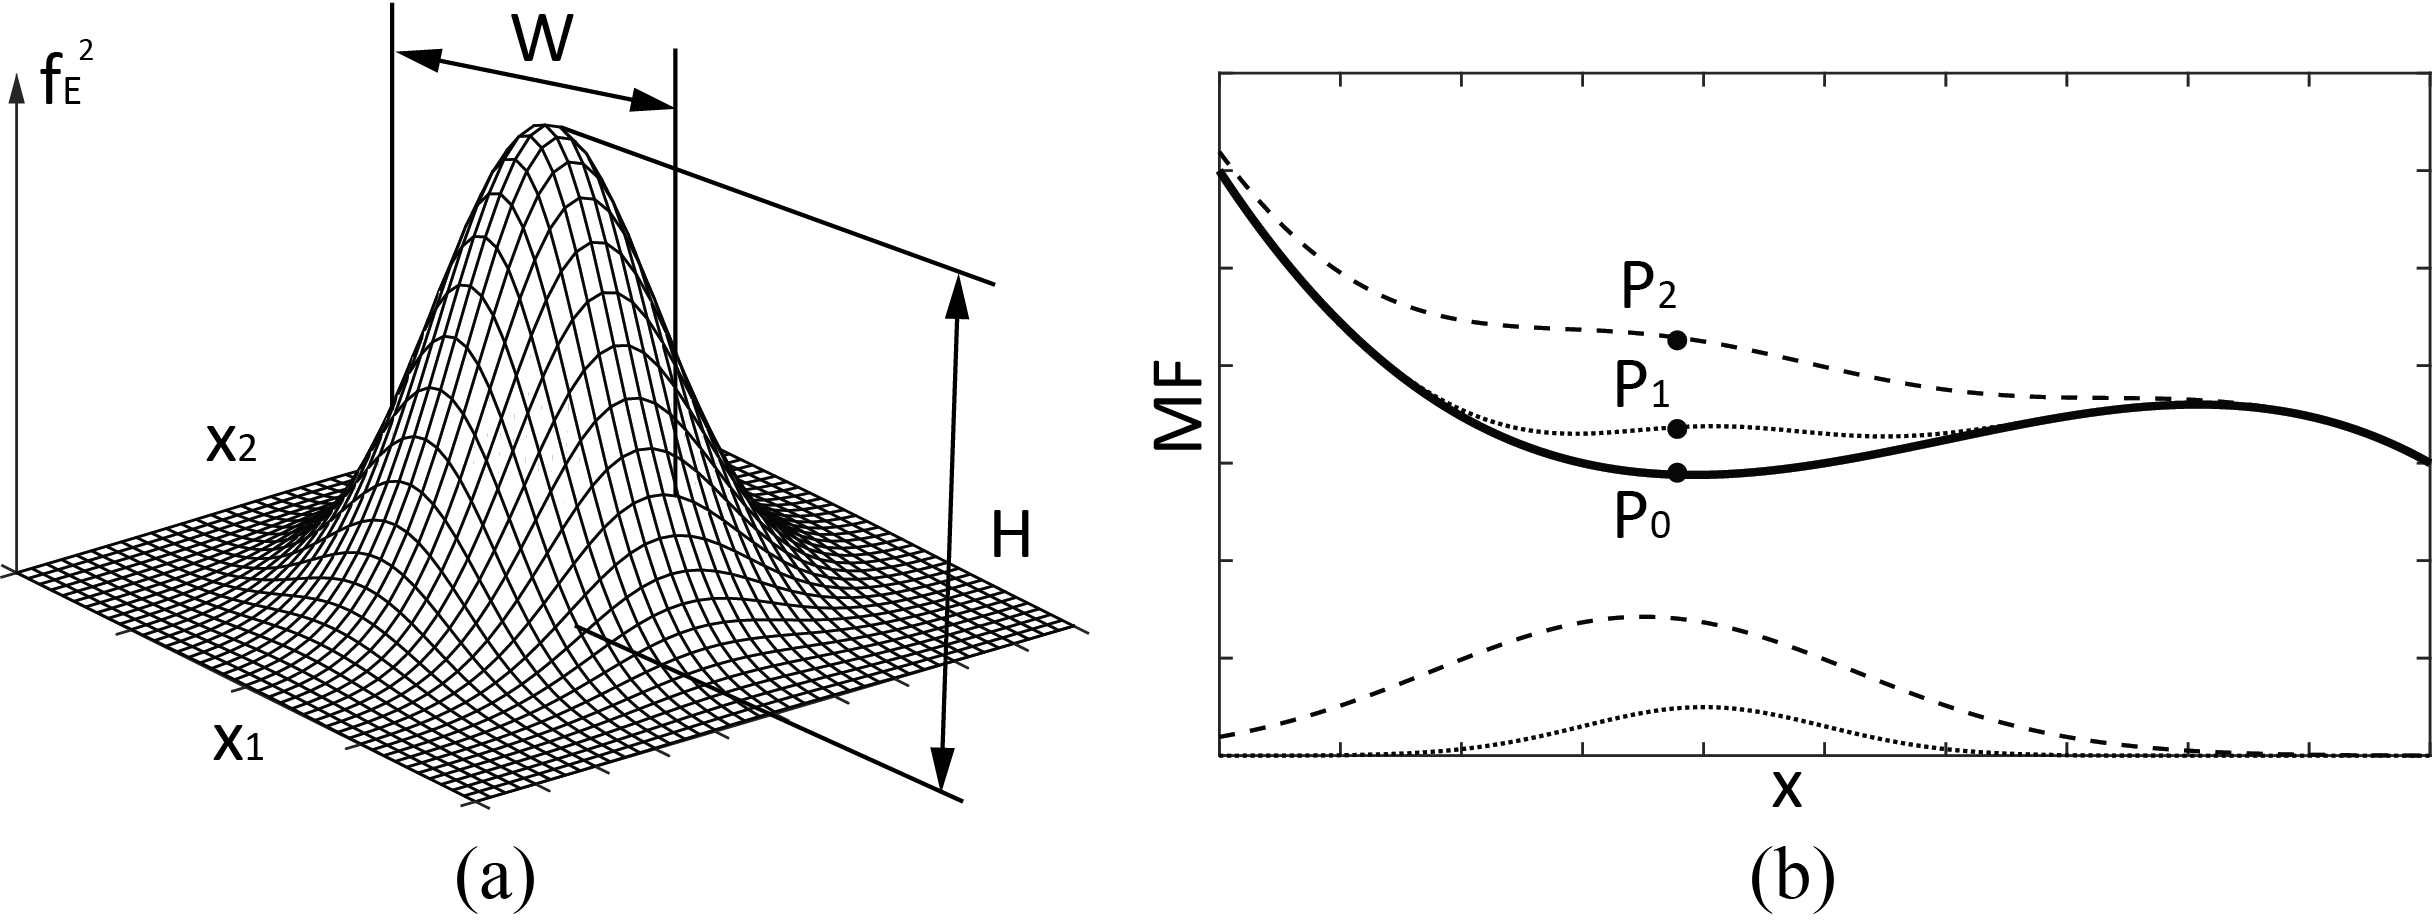
\includegraphics[scale=0.58]{chapter-1/figures/EscapeFunction_explained.png}
    \caption{Explanation of the method of escape function. (a) a 2D escape function illustration, where $H$ modifies the height and $W$ modifies the width of the function. (b) $P_0$ is a minimum for the original 1-D merit function (solid line). By applying escape function (dotted line), $P_0$ is lifted to $P_1$. However, it cannot help the optimizer to escape to a new basin of attraction. When applying a different escape function (dashed line), $P_0$ is lifted to $P_2$. The optimizer escapes to the next basin of attraction.}
    \label{fig: Escape_function_explained}
\end{figure}
Figure \ref{fig: Escape_function_explained}(b) uses a one-dimensional case to illustrate the escape function with two different settings. The solid line represents the original one-dimensional merit function. After local optimization routine, the minimum $P_0$ is obtained. In order to escape from the current basin of attraction, the first escape function setting lifts $P_0$ to $P_1$, as indicated by the dotted line. However, the optimizer remains in the same basin of attraction due to a insufficient modification of the local landscape. The second escape function setting lifts $P_0$ to $P_2$. When local optimization routine applied for $P_2$, the optimizer escapes from the original basin of attraction. In practice, an automatic feedback loop is designed to adjust the escape function settings to increase the efficiency for minimum searching \cite{Isshiki1998}.


\subsubsection{Generic Algorithm}

The genetic algorithm is inspired by the process of natural selection which belongs to the larger class of evolutionary algorithm. Similar to biological reproduction, the genetic algorithm defines population in the optimization landscape. Crossover and mutation occur among the population through generations. The fitness of survival of a given individual is determined within the population. Individuals that have a high fitness will be selected by the algorithm.

In the context of optical design and optimization, the merit function value of an optical system configuration is equivalent to its fitness of survival. Solutions to optical systems are thought of as particular individuals of a hypothetical form of life \cite{Moore1999}. Variables can be compared to genes. The genes are represented by binary codes, which correspond to different variable values \cite{GAreview2018}. 

To initialize an optimization process by genetic algorithm, starting population is created in the optimization landscape. Two kinds of evolutionary activities are considered: crossover and mutation. Crossover happens when the genetic codes of the selected parents are exchanged. Mutation happens when the genetic codes randomly change for individuals. Multiple strategies for crossover and mutation are available. However, trial and error are often needed to determine these strategies. The exit criteria for the genetic algorithm is usually determined by the number of generation the population evolves. 

Different from the method of simulated annealing or escape function, genetic algorithm begins with sampling a larger range of the optimization landscape. Information in different part of the optimization landscape are exchanged to search for the global optimum. However, because of its combinatorial nature, the convergence to a minimum in the continuum variable space is not efficient. Hybrid algorithms where genetic algorithm combined with local optimizer (e.g. damped-least square) is thus recommended to improve the efficiency \cite{Moore1999}.

\subsubsection{Particle Swarm Optimization}
Particle swarm optimization was introduced as an analogue for the interaction of individuals in a swarm or a flock of birds. A collection of candidate solutions, called particles, move around in the optimization space according to simple mathematical rules. The goodness of a particle's location is given by the value of the merit function. For each particle, three vectors are used to represent it in the optimization space: the current location of the particle, the velocity of the particle , and its previous best position. During each iteration, every particle moves from its original location to a new location considering the velocity vector and the best location vectors.  After sufficient iterations, the swarm as a whole is likely to move close to an optimum in the optimization landscape \cite{MenkeParticleSwarm} . 

Similar to the genetic algorithm, particle swarm optimization starts with initializing a population randomly located in the optimization space. Each particle starts with an initial velocity. The position vector and velocity vector of the particles are updated after each iteration as the particles move. Parameters associated with the particle movement such as initial velocity, movement inertia, and acceleration with respect to the global best positions need to be determined based on trial and error. 

As for optical design, each system configuration represents a particle in the optimization space. Particle swarm optimization has been demonstrated in several design cases and it is especially helpful in handling large number of variables such as freeform systems \cite{MenkeParticleSwarm}. On the other hand, hybrid algorithm of combing particle swarm optimization with local optimizer has been proposed \cite{Guo:sParticleSwarm}: particle swarm optimization is used for the discrete optimization of the optical material choices, while the local optimizer is applied to obtain the minimum given the selected material choice.  

\subsection{Saddle Point Method}
In additional to minimum and maximum, saddle point is also a type of stationary points existing in the optimization landscape. Gradient vanishes at all stationary points. When computing the eigenvalues of the Hessian matrix of these stationary point, a minimum has its signs of the eigenvalues all positive, a maximum has its signs of the eigenvalues all negative, and the saddle point has both positive and negative signs of its eigenvalues. Morse Index is defined as the number of the negative signs of the eigenvalues, and the Morse Index of a saddle point is always bigger than \textit{1}. For example, if there is one negative eigenvalue of the Hessian matrix for a stationary point, it is then a saddle point with a Morse Index value of \textit{1}. For a \textit{N}-dimensional optimization landscape, the Morse Index value of its saddle points can vary from \textit{1} to \textit{N-1}.  The value of the Morse Index indicates the number of directions, following the eigenvectors, from which the merit function value decreases. An example of a saddle point in the \textit{2}-dimensional landscape is given in Figure \ref{fig: saddle_illustration}(a). 

Figure \ref{fig: saddle_illustration}(b) shows an example of a \textit{2}-dimensional landscape. If we use an analogue of a mountain view scenario, minima are the \textit{bottom} of the valleys and maxima are the \textit{top} of the hills. Saddle points are located on the passes between the valleys. 

\begin{figure}
    \centering
    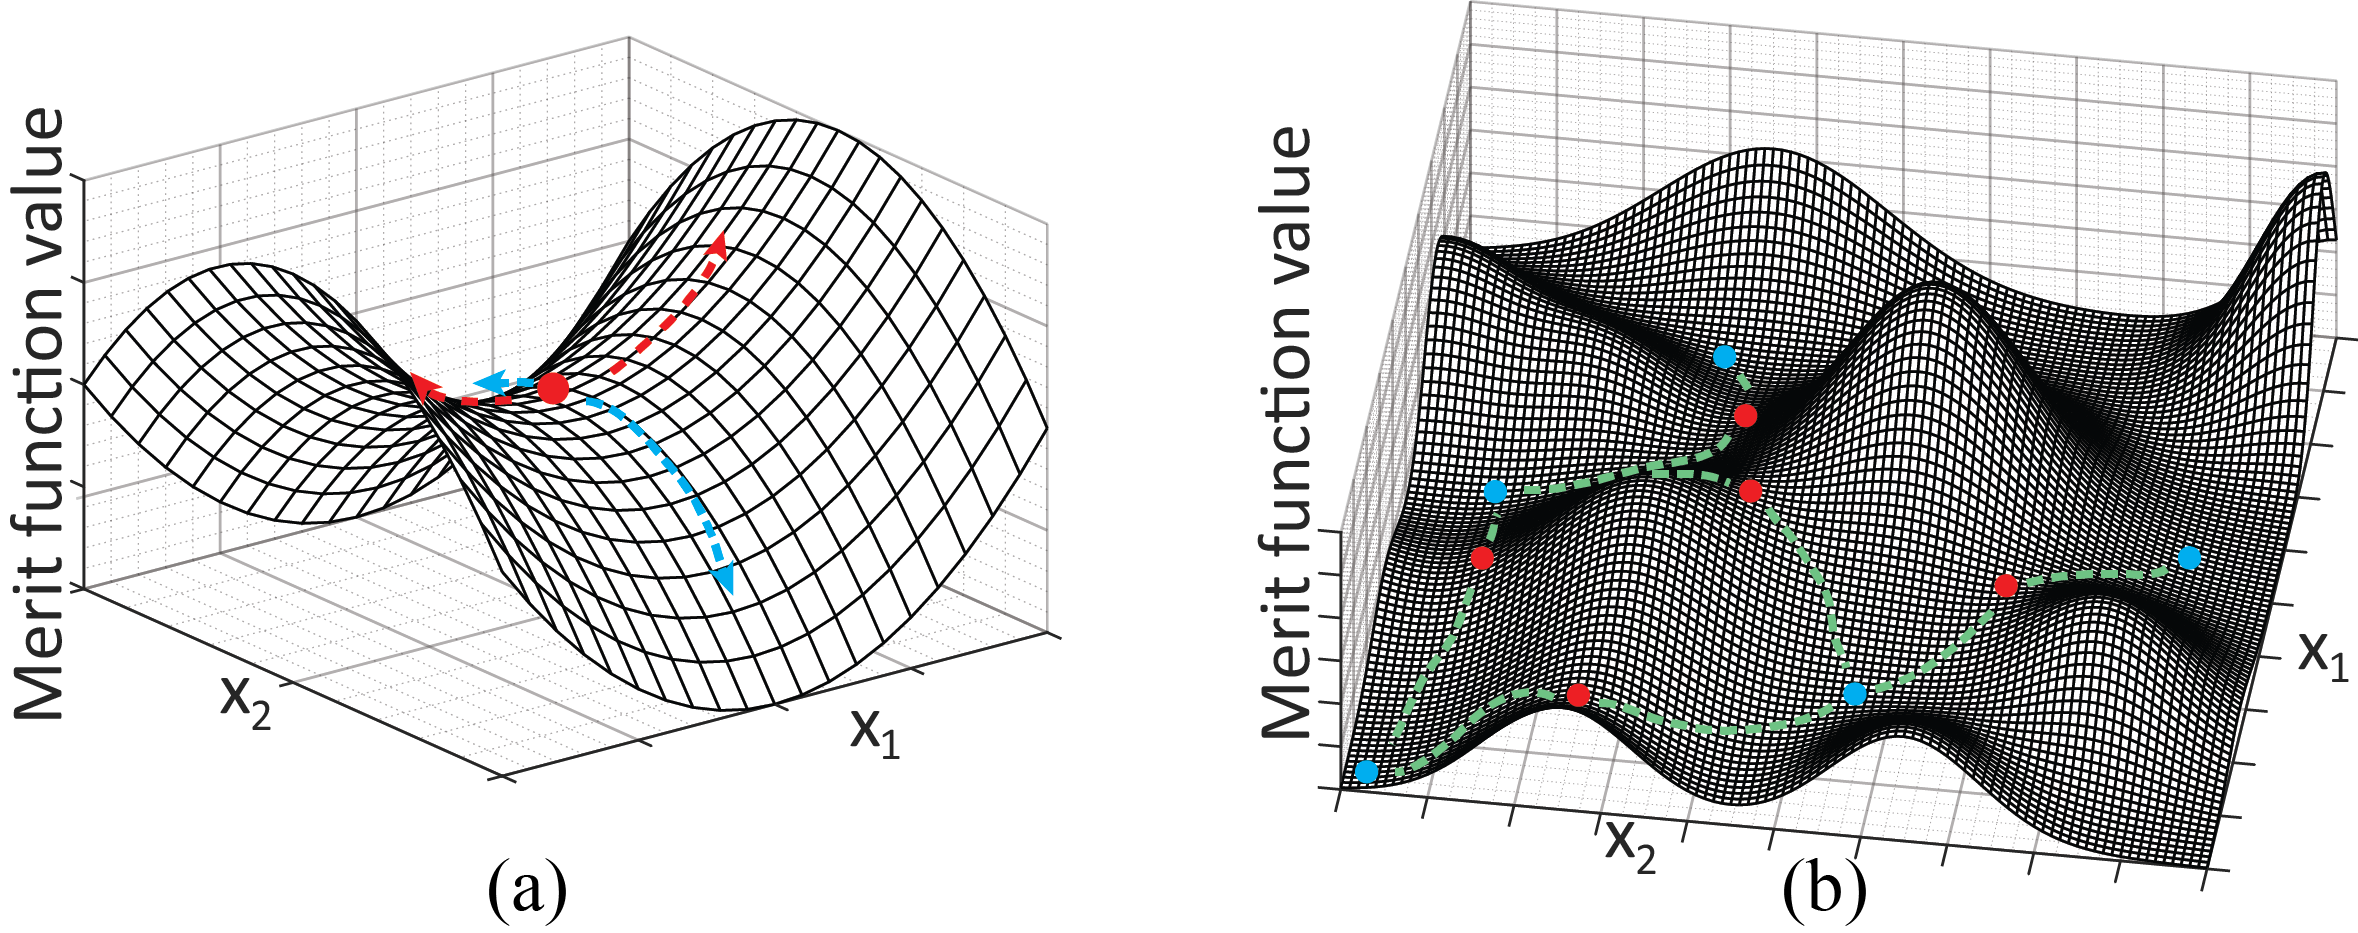
\includegraphics[scale=0.58]{chapter-1/figures/saddle_point_plotted.png}
    \caption{Illustration of the 2D saddle points. (a) A 2D saddle point (horse saddle, with a Morse Index value of 1). It s a maximum in one direction and a minimum along the other direction. (b) Example of a 2D landscape where minima are connected via saddle points. }
    \label{fig: saddle_illustration}
\end{figure} 

The aforementioned global optimization methods treat the optimization landscape as difference basins of attraction. When a larger number of basins are covered, the chance of obtaining a global solution increases. Methods such as simulated annealing and escape function apply strategies to switch basins of attraction when a local minimum is encountered. Methods such as genetic algorithm and particle swarm start with a population distributed in the optimization space. Strategies were applied to search for the basin with the best fit minimum. As a result, the task of searching for local minima can be then replaced by the task of searching for basins of attraction. Saddle point is of special interest when the task is to search for different basins of attraction. As indicated in Figure \ref{fig: saddle_illustration}(b), saddle points with a Morse Index of \textit{1} are located at the boundaries between different basins. Once such a saddle point is found, two basins of attraction can be reached afterwards.

\subsubsection{Saddle Point Detection \label{method: spd}}

NETwork of Local MINima (NETMIN), a tool developed in Delft University of Technology, detects saddle points with Morse Index 1 in the optimization landscape. NETMIN uses constrained local minimization to search saddle points starting from a local minimum. As illustrated in Figure \ref{fig: spd_illustration}, a set of directions is defined around a local minimum. These directions can be determined by the eigenvectors of the Hessian matrix, which are computed at the local minimum. Around the local minimum, the surfaces along which the merit function is constant have the shape of ellipsoids \cite{MarinescuSPD07}. The eigenvectors of the Hessian matrix correspond to the directions of the half-axes of the ellipsoids. Along each direction, a set of hyperplanes which orthogonal to the direction vector can be defined. For $N$-dimensional space, these hyperplanes have a dimension of $N-1$. The distance between the local minimum and the hyperplane is indicated by $t$. On each hyperplane, a constrained minimization can be performed. The positions of the constrained minima as a function of  $t$ is symbolically shown in Figure \ref{fig: spd_illustration}(a). The merit function value ($MF$) as a function of $t$ is shown in Figure \ref{fig: spd_illustration}(b). When $t$ is sufficiently small, the merit function value of the constrained minimum on the hyperplane increases. At a certain $t = t_{max}$, the merit function value reaches its maximum value (point $s$ in Figure \ref{fig: spd_illustration}(a)). This point is a maximum along the vector direction and a minimum on the $(N-1)$-dimensional hyperplane, hence a saddle point with Morse Index 1.  

\begin{figure}
    \centering
    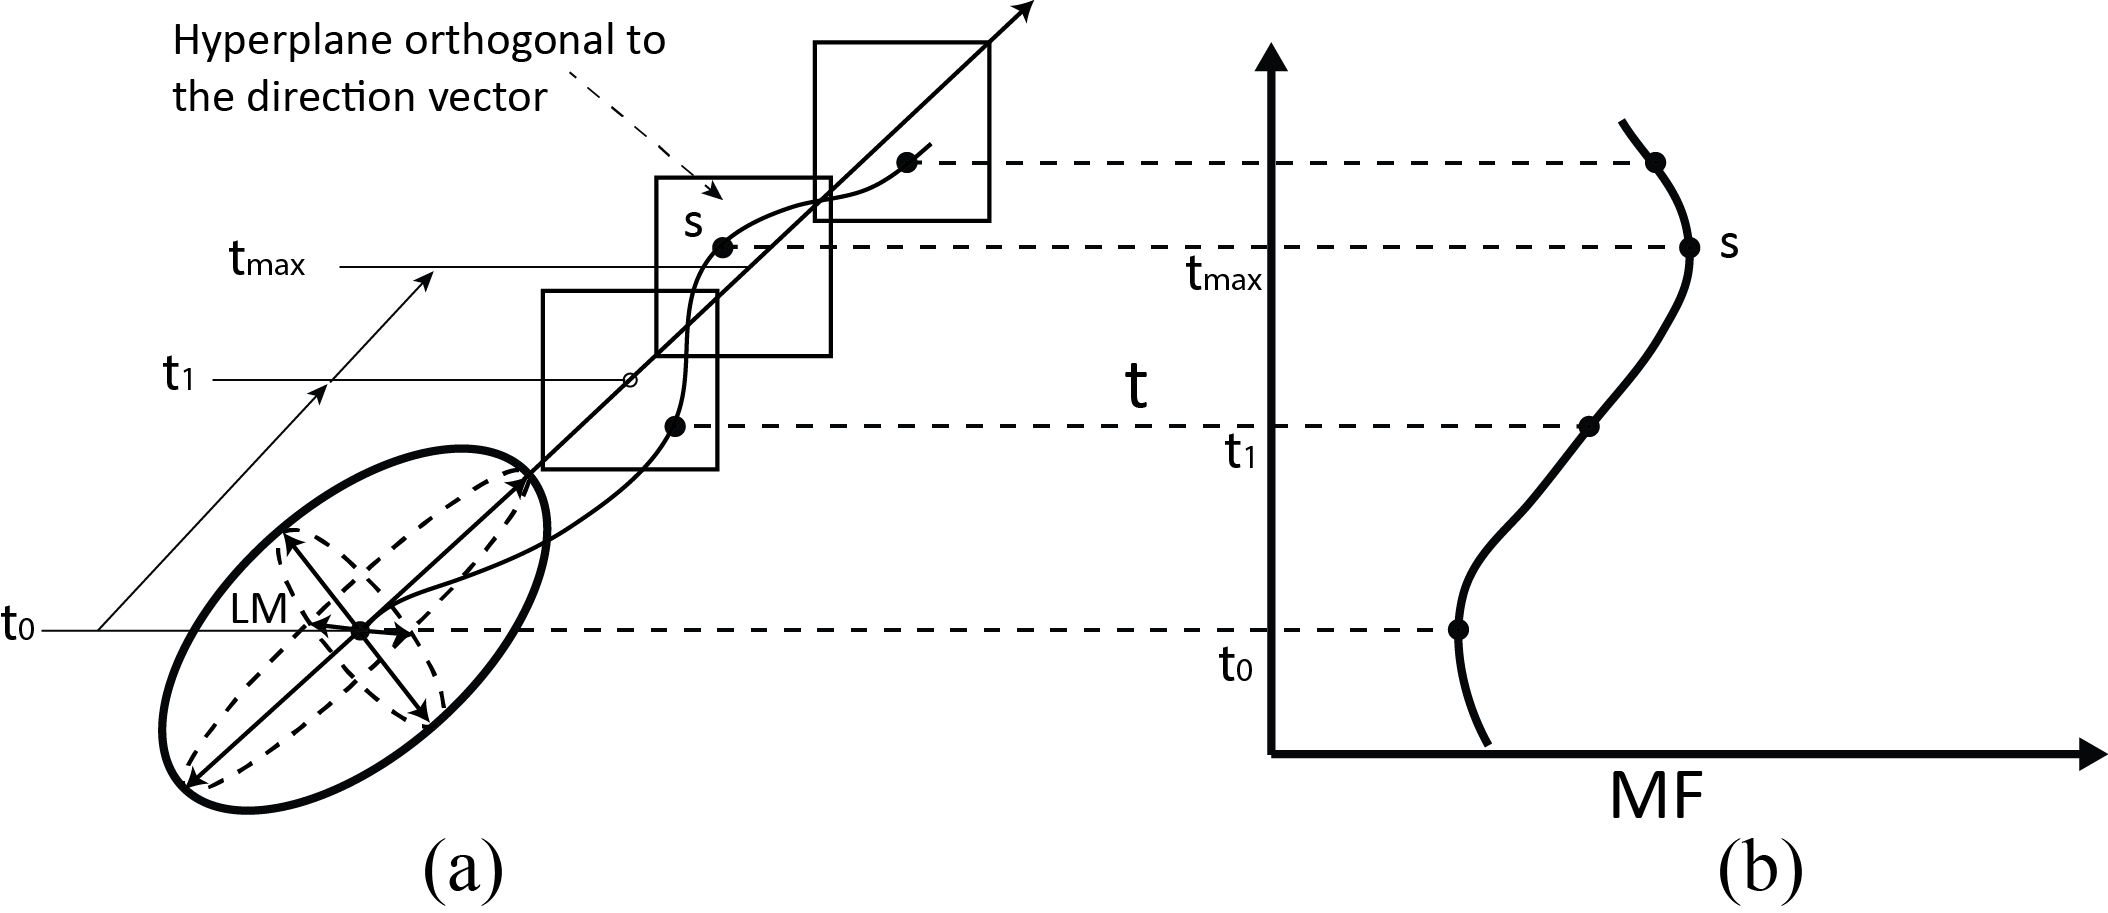
\includegraphics[scale=0.58]{chapter-1/figures/spd_plot.png}
    \caption{Illustration of constrained optimization to detect saddle point in the optimization landscape. (a) Saddle point detection in high-dimensional space. Minimization is performed on hyper-planes which are orthogonal to the chosen direction. (b) Example of MF value along a search direction. The saddle point detection starts from an existing local minimum. The directions around the local minimum are chosen towards the directions of the eigen vectors of the Hessian matrix. The value of the MF will first increase. After finding the saddle point, the MF value will decrease. }
    \label{fig: spd_illustration}
\end{figure} 

When a saddle point with Morse Index 1 is detected, a point "on the other side" of the saddle point can be chosen to start a local optimization routine. The optimizer searches in a different basin of attraction to find a new local minimum. NETMIN combines local optimizer and saddle point detection algorithm to reveal the network of local minima and saddle point in the optimization landscape. NETMIN has been used to study triplet network (\cite{PascalTriplet2009}) and six-mirror systems (\cite{MarinescuSPD07}). In Chapter \ref{chapter_SPC_simple_system_landscape} of this thesis, we also use NETMIN obtained results as a reference. 

The computation of NETMIN is expensive. For each step along the chosen direction, a constrained optimization has to be performed. In practice, multiple directions have to be searched to find all saddle points around a local minimum. Parallel processing can be enabled to facilitate the search.  


\subsubsection{Saddle Point Construction }
In the context of lens design, research has shown that saddle point can be constructed directly instead of performing a saddle point detection algorithm \cite{vanTurnhoutThesis2009} \cite{MVTurnhoutSPC15}. It was firstly found that the saddle point systems obtained via the saddle point detection algorithm always contains low power meniscus lenses. Once the thickness of these meniscus are reduced to zero, it is possible to show that the these systems becomes a saddle point in the design landscape (detailed explanation is given in Chapter \ref{chapter_SPC_method_reccomendation}).

An illustration of the saddle point construction is given in Figure \ref{fig: spc_illustration}. The construction of a saddle point is indicated by step 1 and 2: It starts from a local minimum and adds an extra lens element to the existing system. When a saddle point system is obtained in step 2, step 3 and step 4 show how to obtain two new local minima from the saddle point system. The detailed explanation of saddle point construction is given in Chapter \ref{chapter_SPC_method_reccomendation}. 

\begin{figure}
    \centering
    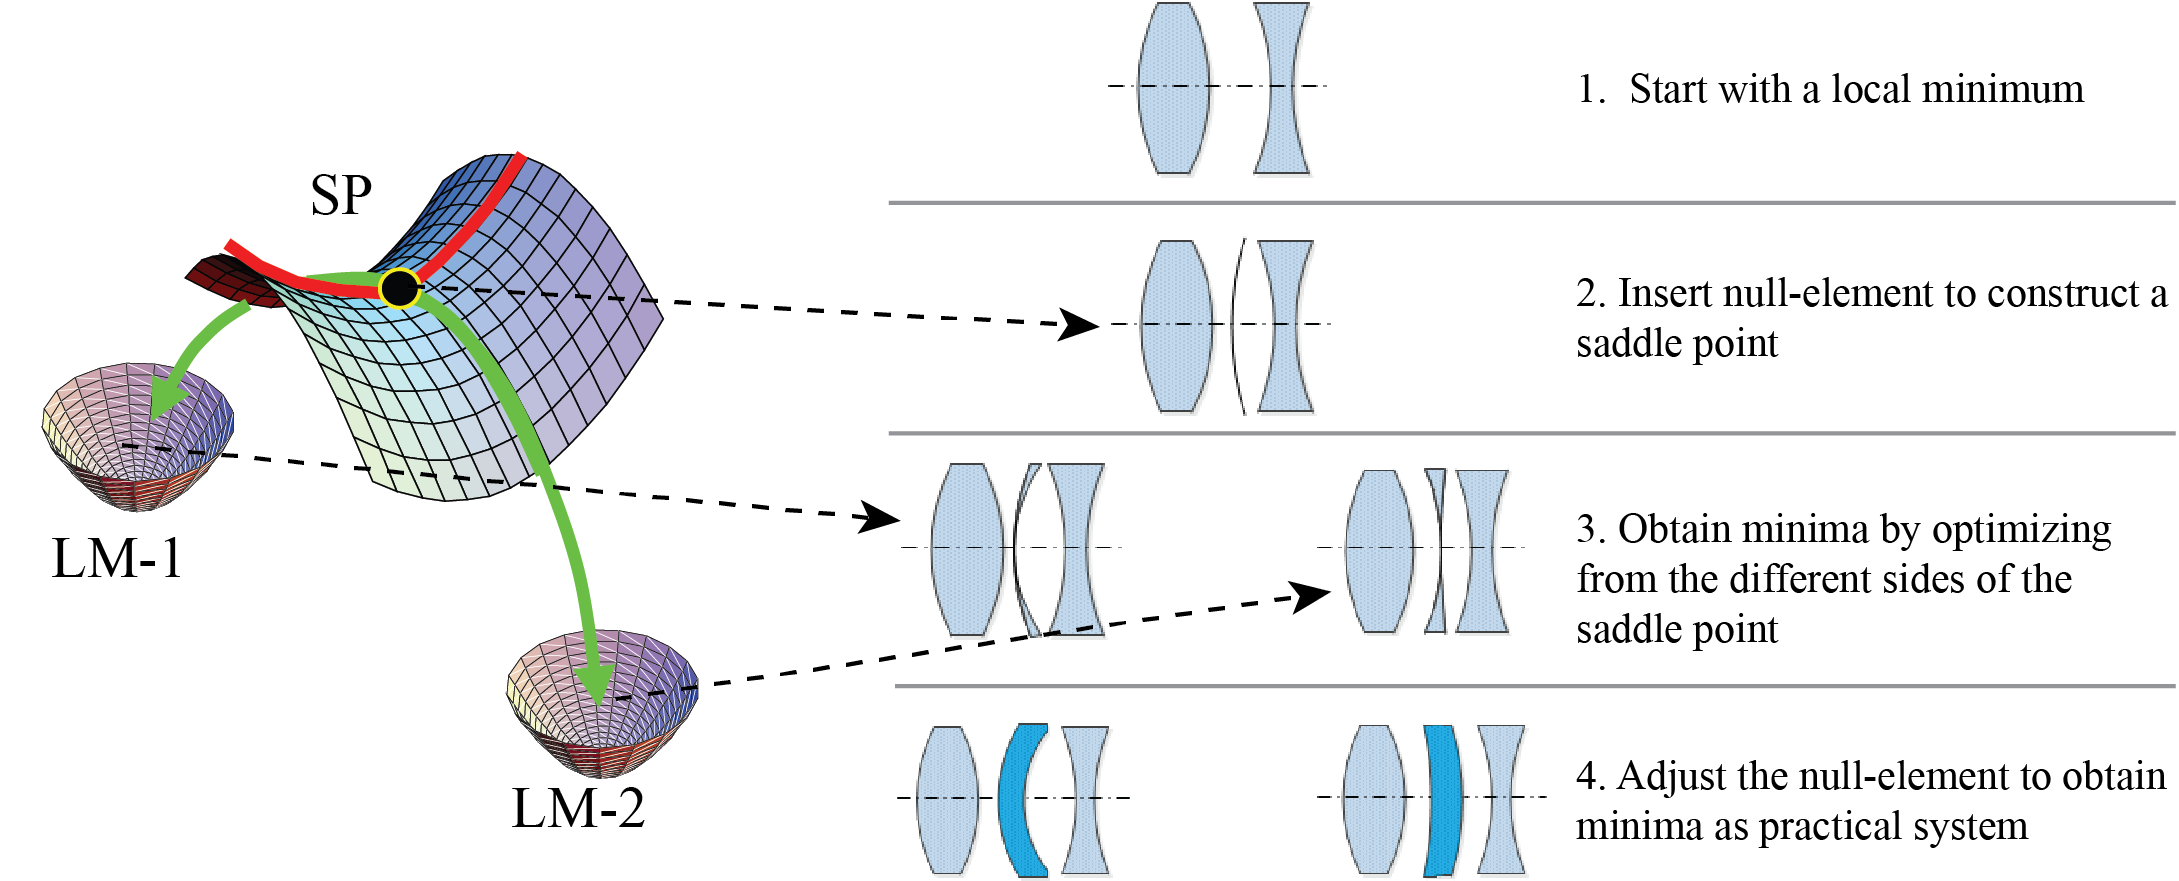
\includegraphics[scale=0.58]{chapter-1/figures/spc_illustrate.png}
    \caption{Illustration of the saddle point construction process. The right side shows an example of constructing a saddle point on a doublet minimum. Two triplet minima result from this process. The left is an example of how a saddle point leads to two minima in a 2D optimization space. In step 2 and 3, the optimization space remains static. In step 1 and 2, the optimization space has different dimensions (step 1 does not include the null-element, and step 4 adds extra variables). }
    \label{fig: spc_illustration}
\end{figure} 

% the next chapter is dedicated to saddle point construction. In this part, it is sufficient to introduce the topic.

% what is added research value of this thesis

%%%%%%%%%%%%%%%%%%%%%%%%%% SECTION 5 %%%%%%%%%%%%%%%%%%%%%%%%%%%%%%%%%%%%%%%%%%%%%%%%%%%%%%%%
\section{Conclusion}
In this chapter, we use the example of a magnifying glass to demonstrate how a lens can be designed on paper. However, nowadays the optical systems are getting too complicated to perform such analysis and be designed from scratch. 

The major concept such as basins of attraction, starting point, local and global optimization are explained for the optimization part of lens design. We show that the optimization algorithms reply almost exclusively on generally applicable mathematical models and uses little or no specific knowledge about the optical system (and its design landscape). We briefly mentioned SPC at the end and the special structure of the lens design landscape it reveals. In the following three chapters, we will focus on the SPC method and its effectiveness in different design scenarios. 

\references{dissertation}

\begin{comment}

%%%{BACK-UPS
\subsection{Backup notes}
where to insert the lens -> combine with experience 
whether the result is satisfactory -> judge by experience 
controlled way of the getting the solution 

Neural network? 
It is a hot topic so it is good to also mention something about the Neural network work. 
\cite{JM_nn_93}  \cite{Yang:19} \cite{Cote:19}

\section{Problem for optical system design}

When designing an optical system, it is always necessary to consider its source and receiver. When designing imaging system, the object represents the source, where lights from all angles are emitting from the object at each point. The receiver is usually called image, which is normally a flat plane (such as a photosensitive film, or a charged-carrier device sensor). The optical system is located between the source and receiver, after which the light will arrive at the receiver with a designed performance instead of propagate in the air. The source and receiver in a non-imaging system can have more variety: a source can be a simple point source, or can be an extended source with a certain geometrical shape. The receiver can be all kinds of 3D-shape. 

An optical design problem uses all the available components which manipulate the light in a way that it will achieve a certain purpose as the designer desired. This can be either imaging, to focus a point in the object side to the image side with the maximal retained information, or can be non-imaging, to distribute the energy of the light in a way for a certain purpose, such as creating a homogeneous illumination. 

When mentioning optical design, the term is not specified enough. It should be including all the possible way of designing with manipulating light to achieve certain purpose. Regardless of the using of the components or the scale of the components. 

Optical design components, polarizer, diffractive components, multiple aperture (light field camera, cell-phone camera).

The design case mainly handled in this thesis is the imaging system design, in particular with optical lens design. In this case, the used components are mainly 

\end{comment}


